\documentclass[a4paper, 14pt, fleqn]{extarticle}
\usepackage{float}
\usepackage[justification=centering]{caption}
\usepackage{fefutitle}
\usepackage{kotlinlisting}

\begin{document} 
	\fefutitle{3}
	
	
	\pagebreak
	\section{Введение}
		В данной лабораторной работе мне нужно решить с помощью систем компьютерной математики 5 дифференциальных уравнение 1-го порядка и 3 2-го порядка, реализовать метод Эйлера на ЯП <<Kotlin>>.

	\pagebreak
	\section{Задание 1}
		\subsection{Постановка задачи}
			\noindent Для следующих дифференциальных уравнений указать вид, дать характеристику, найти общее
			решение с помощью программ компьютерной математики:
		\begin{enumerate}
			\item \( y' + e^{y'} = \ln{x} \)
			\item \( y = xy' - x^2 \cdot y'^{3} \)
			\item \( \tan{\dfrac{y}{y'}} = \ln{y} \)
			\item \( xy'^3 - yy'^2 + 1 = 0 \)
			\item \( xy' \cdot (y' + 2) = y \)
		\end{enumerate}
		\subsection{Решение}
			\noindent Поиск решения будет проводиться в системе компьютерной математики Wolfram Mathematica.
			\begin{enumerate}
				\item \(  y' + e^{y'} = \ln{x} \)

					\textit{Вид уравнения:} \( x = F(y') \)

					\textit{Характеристика:} Неразрешенное относительно производной, не содержит функцию
		
					\textit{Ответ:} \(\begin{cases}
									x = e^{p+e^p}, \\
									y = e^{e^p}(1+e^p) + C;
								\end{cases}\) 
				\item \(  y = xy' - x^2 \cdot y'^{3} \)

					\textit{Вид уравнения:} \( y = F(x, y') \)

					\textit{Характеристика:} Неразрешенное относительно производной
		
					\textit{Ответ:} \(\begin{cases}
									x = Cp^{-\frac{3}{2}} - p^{-2}, \\
									y = xp(1-x);
								\end{cases}\) 

				\item \( \tan{\dfrac{y}{y'}} = \ln{y} \)
				
					\textit{Вид уравнения:} \( y' = F(y) \)
 
					\textit{Характеристика:} Уравнение c разделяющимся переменными

					\textit{Ответ:} \( 2\ln{y} \cdot \arctan{\ln{y}} -\ln{\big(\ln^2{y} + 1\big)} - 2x = C \)

				\item \( xy'^3 - yy'^2 + 1 = 0 \)

					\textit{Вид уравнения:} \( y = F(x, y') \)

					\textit{Характеристика:} Уравнение Клеро
		
					\textit{Ответ:} \( y = Cx + \dfrac{1}{C^2} \)

				\item \( xy' \cdot (y' + 2) = y \)

					\textit{Вид уравнения:} \( y = F(x, y') \)

					\textit{Характеристика:} Квадратное относительно \( y' \)
		
					\textit{Ответ:} \(\begin{cases}
									x = \dfrac{C}{p^2}, \\
									y = xp(p+2);
								\end{cases}\) 
			\end{enumerate}

	\pagebreak
	\section{Задание 2}
		\subsection{Постановка задачи}
			\noindent Разрешить следующие уравнения относительно производной и, используя метод Эйлера, найти значение функции в точке.
 					Нарисовать график искомой функции. Реализацию решения проводить на языке <<Kotlin>>:
			\begin{enumerate}
				\item \( e^{x-y} = \cos{\big(y'\sin{x} - \tan^2{(\sec{xy})} - \tan{y}\big)}; \)

					\( y\bigg(\dfrac{\pi}{3}\bigg) = \ln{7},\ y(1) = ? \)

				\item \( xy' - y^2 \cdot e^{-y^2} = \sin{\pi x}; \quad y(1) = \ln{2},\  y{(\pi)} = ?\)
			\end{enumerate}
		\subsection{Решение}
				\begin{enumerate}
					\item \( e^{x-y} = \cos{\big(y'\sin{x} - \tan^2{(\sec{xy})} - \tan{y}\big)}; \)

						\( y\bigg(\dfrac{\pi}{3}\bigg) = \ln{7},\ y(1) = ? \)
						
						\( y' = \dfrac{\arccos{(e^{x-y})} +  \tan^2{(\sec{xy})} + \tan{y}}{\sin{x}} \)

						\( y\bigg(\dfrac{\pi}{3}\bigg) = \ln{7},\ y(1) \approx 1.97059 \)

						\begin{figure}[H]
						    	\centering
						    	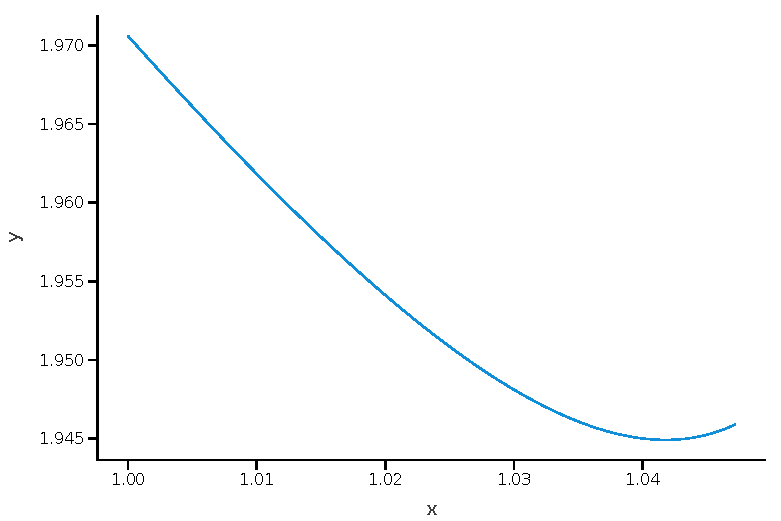
\includegraphics[width = .7\linewidth]{plot2.pdf}
						   	\caption[.] {Метод Эйлера для \linebreak \( e^{x-y} = \cos{\big(y'\sin{x} - \tan^2{(\sec{xy})} - \tan{y}\big)}\)}
  						\end{figure}
					\item  \( xy' - y^2 \cdot e^{-y^2} = \sin{\pi x}; \quad y(1) = \ln{2},\  y{(\pi)} = ?\)

						\( y' = \dfrac{\sin{\pi x} + y^2 \cdot e^{-y^2}}{x} \)

						\(  y(1) = \ln{2},\  y{(\pi)} \approx 0.78616 \)

						\begin{figure}[H]
						    	\centering
						    	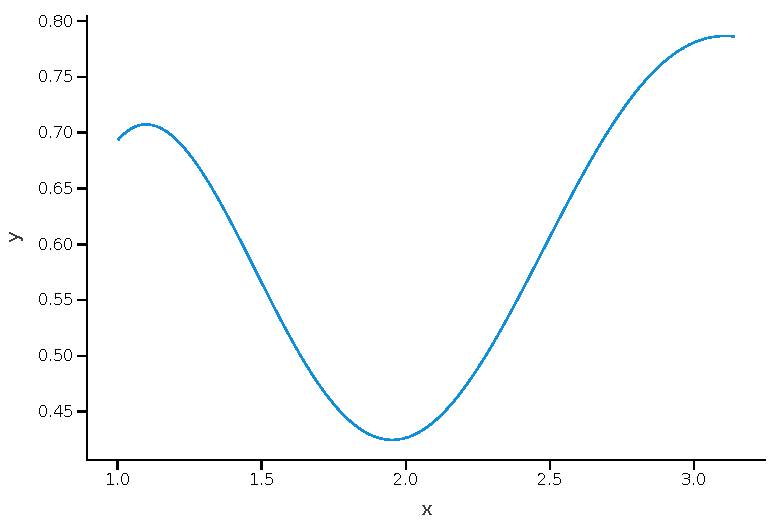
\includegraphics[width = .7\linewidth]{plot1.pdf}
						   	\caption[.] {Метод Эйлера для \linebreak \( xy' - y^2 \cdot e^{-y^2} = \sin{\pi x} \)}
  						\end{figure}	
				\end{enumerate}
		\subsection{Код программы}
			\begin{lstlisting}[language=Kotlin]
import jetbrains.letsPlot.export.ggsave
import jetbrains.letsPlot.geom.*
import jetbrains.letsPlot.letsPlot
import kotlin.math.ln

data class Point (
    var x: Double,
    var y: Double,
)

fun task_1(x: Double, y: Double): Double {
    return ((Math.sin(Math.PI*x) + Math.pow(y, 2.0)
            * Math.pow(Math.E, -1 * Math.pow(y, 2.0)))/x)
}

fun task_2(x: Double, y: Double): Double {
    return (Math.acos(Math.pow(Math.E, x-y))
            + Math.pow(Math.tan(1/Math.cos(x*y)), 2.0)
            + Math.tan(y))/Math.sin(x)
}

fun plot(function: (Double, Double) -> Double,
         p: Point, plot_name: String,
            x_end: Double, n: Int){
    val xs = mutableListOf<Double>()
    val ys = mutableListOf<Double>()
    val h = (x_end - p.x) / n
    for (i in 0..n) {
        p.y += h * function(p.x, p.y)
        p.x += h
        xs.add(p.x)
        ys.add(p.y)
    }
    print(p.y)
    val data = mapOf<String, Any>(
        "x" to xs,
        "y" to ys,
    )
    val fig = letsPlot(data) {x = "x"; y="y"} 
+ geomLine()
    ggsave(fig, plot_name)
}

fun main() {
    val p_1 = Point(1.0, ln(2.0))
    val p_2 = Point(Math.PI/3, ln(7.0))
    plot(::task_1, p_1, "plot1.svg", Math.PI, 1000000)
    plot(::task_2, p_2, "plot2.svg", 1.0, 1000000)
}
				\end{lstlisting}

	\pagebreak
	\section{Задание 3}
		\subsection{Постановка задачи}
			\noindent Для следующих дифференциальных уравнений определить тип, дать характеристику и найти общее решение с помощью программ компьютерной математики:
		\begin{enumerate}
			\item \( xy'' - y' \cdot (xy' \cdot \tan{y} + 1) = 0\)
			\item \( y'^3 = e^{\frac{1}{y'}}y'' \)
			\item \( y'' \cdot e^y + 2y' = y'^2 \cdot e^y \)
		\end{enumerate}
		\subsection{Решение}
			\noindent Поиск решения будет проводиться в системе компьютерной математики Wolfram Mathematica.
			\begin{enumerate}
				\item \(  xy'' - y' \cdot (xy' \cdot \tan{y} + 1) = 0 \)

					\textit{Вид уравнения:} \( F(x, y, y', y'') = 0 \)

					\textit{Характеристика:} Уравнение в полных производных
		
					\textit{Ответ:} \( 2\sin{y} = C_1 - C_2x^2 \)

				\item \( y'^3 = e^{\frac{1}{y'}}y'' \)
					
					\textit{Вид уравнения:} \( F(y', y'') = 0 \)

					\textit{Характеристика:} Интегрируемое уравнение
		
					\textit{Ответ:} \(x =  (y - C_1) \cdot \ln{( C_1 - y )}  - y + C_2\)

				\item \( y'' \cdot e^y + 2y' = y'^2 \cdot e^y \)
				
					\textit{Вид уравнения:} \( F(y, y', y'') = 0 \)

					\textit{Характеристика:} Общее уравнение
		
					\textit{Ответ:} \( y = \ln{\dfrac{\tan{\big(C_1(x+C_2)\big)}}{C_1}} \)
			\end{enumerate}

	\section{Заключение}
		\noindent Я с помощью Wolfram Mathematica решил 5 дифференциальных уравнений 1-го порядка и 3 2-го, написал программу на языке <<Kotlin>>, реализующую метод Эйлера. Оформлял отчёт по работе  в <<TeX Live>>.

\end{document}